\chapter{Introduction to Formal Semantics}
\label{chap:intro-fs}

Semantics is the study of the meaning of language. In this Chapter, we will
review the very basics of a school of formal semantics which originated
with Richard Montague in the early
70's~\cite{montague1970english,montague1970universal,montague1973proper}~(\ref{sec:montague}). We
then present a formalism that embodies the principles of montagovian
semantics, the Abstract Categorial
Grammars~\cite{de2001towards}~(\ref{sec:acg}). In
Chapter~\ref{chap:dynamic-semantics}, we will be analyzing anaphora in
$\calc$ by emulating theories of dynamic semantics. To that end, we briefly
present dynamic semantics by introducing two of its incarnations: Discourse
Representation Theory~\cite{kamp1993discourse}~(\ref{sec:drt}) and
Type-Theoretic Dynamic Logic~\cite{de2006towards}~(\ref{sec:ttdl}).

\minitoc


\section{Montague Semantics}
\label{sec:montague}

When studying semantics, one of the verifiable predictions that we can make
is whether the contents of one utterance entails the contents of
another. This issue already preoccupied Aristotle, who addressed the
problem in his study of syllogisms. Using his theory, Aristotle could
systematically predict that the contents of
Example~\ref{ex:syllogism-hypothesis} entail the contents of
Example~\ref{ex:syllogism-conclusion}, i.e.\ ``if
(\ref{ex:syllogism-hypothesis}), then (\ref{ex:syllogism-conclusion})'' is
a valid argument.

\begin{exe}
  \ex Every man is mortal. Socrates is a man. \label{ex:syllogism-hypothesis}
  \ex Socrates is mortal. \label{ex:syllogism-conclusion}
\end{exe}

In the 20th century, mathematical logic studied similar properties on
formal artificial languages, leading to the developments of new ideas such
as model theory and Tarski's definition of
truth~\cite{sep-tarski-truth,tarski1986arithmetical}. Montague then argues
that natural languages deserve the same formal treatment as the artificial
languages of logic and mathematics:

\begin{quote}
  There is in my opinion no important theoretical difference between
  natural languages and the artificial languages of logicians; indeed, I
  consider it possible to comprehend the syntax and semantics of both kinds
  of language within a single natural and mathematically precise theory.

  \begin{flushright}
  Universal Grammar~\cite{montague1970universal}
  \end{flushright}
\end{quote}

In formal logic, the formulas of the artificial languages are defined
inductively, by a series of construction rules. The definition of truth is
then inductive on the structure of the formula: for every rule that lets us
form a logical formula, there is a rule which tells us how to compute its
truth value in a model. In his approach, Montague applies the very same
strategy to natural language~\cite{montague1973proper}.


\subsection{Syntax}
\label{ssec:montague-syntax}

Contrary to propositional language, whose language is made only of
propositions, the set of which is given inductively, natural language
expressions fall into many syntactic categories. Montague therefore defines
the expressions of a language as a family of sets, indexed by
categories. The categories are defined inductively as well: $e$ is a
category (of entity-denoting expressions), $t$ is a category (of
truth-denoting expressions) and for every two categories $A$ and $B$,
$A / B$ and $A \doubleslash B$ are categories.\footnote{The meanings of
  these connectives will be given by their use in the grammar, but
  intuitively, $A / B$ is the category of expressions that when combined
  with an expression of category $B$ yield an expression of category $A$,
  and $A \doubleslash B$ is the category of expressions that denote
  functions from the meanings of category $B$ to the meanings of category
  $A$.}  Montague identifies some of the categories which will become
useful in formulating the grammar. In our example, we will make use of the
following four:

\begin{itemize}
\item $IV = t / e$, the category of intransitive verbs
\item $T = t / IV$, the category of terms (i.e.\ noun phrases)
\item $TV = IV / T$, the category of transitive verbs
\item $CN = t \doubleslash e$, the category of common nouns
\end{itemize}

Having established the categories, we will now give some of the
construction rules in Montague's grammar. The sets $P_A$ of phrases of
category $A$ are defined as the smallest sets being closed on the following
constructions rules (taken almost verbatim from~\cite{montague1973proper}):

\begin{description}
\item[S1] $B_A \subseteq P_A$ for every category $A$.

  Here, $B_A$ is the set of \emph{basic expression} of category $A$. For
  the categories that we are interested in, these sets look something like
  this:

  \begin{align*}
    B_{IV} &= \{ \textbf{run}, \textbf{walk}, \textbf{talk}, \ldots \} \\
    B_{T} &= \{ \textbf{John}, \textbf{Mary}, \textbf{Bill}, \textbf{he}_0,
            \textbf{he}_1, \textbf{he}_2, \ldots \}\footnotemark \\
    B_{TV} &= \{ \textbf{eat}, \textbf{love}, \textbf{seek}, \textbf{find},
             \ldots \} \\
    B_{CN} &= \{ \textbf{man}, \textbf{woman}, \textbf{unicorn}, \ldots \}
  \end{align*}

  \footnotetext{$B_{T}$ contains a countably infinite set of $T$-typed
    variables $\textbf{he}_0$, $\textbf{he}_1$, $\textbf{he}_2$, \ldots}

\item[S2] If $\zeta \in P_{CN}$, then
  $F_0(\zeta), F_1(\zeta), F_2(\zeta) \in P_{T}$, where

  \begin{align*}
    F_0(\zeta) &= \textbf{every } \zeta \\
    F_1(\zeta) &= \textbf{the } \zeta \\
    F_2(\zeta) &\text{ is \textbf{a} $\zeta$ or \textbf{an} $\zeta$ according
    as to whether the first word in $\zeta$ takes \textbf{a} or \textbf{an}}
  \end{align*}

\item[S4] If $\alpha \in P_{t / IV}$\footnote{i.e.\ $\alpha \in P_{T}$}
  and $\delta \in P_{IV}$, then $F_4(\alpha, \delta) \in P_{t}$, where
  $F_4(\alpha, \delta) = \alpha \delta'$ and $\delta'$ is the result of
  replacing the first verb in $\delta$ by its third-person singular
  present.

\item[S5] If $\delta \in P_{IV / T}$\footnote{i.e.\ $\delta \in P_{TV}$}
  and $\beta \in P_{T}$, then $F_5(\delta, \beta) \in P_{IV}$, where
  $F_5(\delta, \beta) = \delta \beta$ if $\beta$ does not have the form
  $\textbf{he}_n$ and $F_5(\delta, \textbf{he}_n) = \textbf{him}_n$.

\item[S14] If $\alpha \in P_{T}$ and $\phi \in P_{t}$, then
  $F_{10,n}(\alpha, \phi) \in P_{t}$, where either:

  \begin{itemize}
  \item $\alpha$ does not have the form $\textbf{he}_k$, and
    $F_{10,n}(\alpha, \phi)$ comes from $\phi$ by replacing the first
    occurrence of $\textbf{he}_n$ or $\textbf{him}_n$ by $\alpha$ and all
    other occurrences of $\textbf{he}_n$ or $\textbf{him}_n$ by
    $\textbf{he}$/$\textbf{she}$/$\textbf{it}$ or
    $\textbf{him}$/$\textbf{her}$/$\textbf{it}$ respectively, according to
    whether the first noun in $\alpha$ is masculine/feminine/neuter, or
  \item $\alpha = \textbf{he}_k$, and $F_{10,n}(\alpha, \phi)$ comes from
    $\phi$ by replacing all occurrences of of $\textbf{he}_n$ or
    $\textbf{him}_n$ by $\textbf{he}_k$ or $\textbf{him}_k$
  \end{itemize}
\end{description}

Note that Montague maintains a distinction between deep syntax
(tectogrammar) and surface syntax (phenogrammar). For example, the rule S4
tells us that a noun phrase $\alpha \in P_{t / IV}$ can be combined with an
intransitive verb $\delta \in P_{IV}$ to yield a sentence
$F_4(\alpha, \delta)$ (this is tectogrammar). Then, the definition of $F_4$
tells us that the noun phrase should precede the verb phrase and that the
verb phrase should be in third-person singular present\footnote{All the
  noun phrases in this fragment are third-person singular.} (this is
phenogrammar). Similarly for the rule S5, it tells us that a transitive
verb $\delta \in P_{IV / T}$ can be combined with a noun phrase
$\beta \in P_{T}$ to form an (intransitive) verb phrase
$F_5(\delta, \beta)$. The definition of $F_5$ then tells us that such a
verb phrase is pronounced/written with the transitive verb first and the
noun phrase second and that the noun phrase should be in accusative
form. In S2, this is the case as well. The rule tells us that for every
noun $\zeta \in P_{CN}$, there are the universal, definite and indefinite
noun phrases $F_0(\zeta)$, $F_1(\zeta)$ and $F_2(\zeta)$ respectively. The
definitions of $F_0$, $F_1$ and $F_2$ then give us the surface realizations
of these noun phrases.\footnote{If we were to write a grammar of French, we
  would keep the same tectogrammar and just replace the definitions of
  $F_0$, $F_1$ and $F_2$ to use $\textbf{chaque}$,
  $\textbf{le}$/$\textbf{la}$/$\textbf{l'}$ and
  $\textbf{un}$/$\textbf{une}$.}

Using the grammar given above, we can derive, e.g., the sentence
\textbf{John seeks a unicorn}. We can record the rules we have used when
constructing the sentence in a \emph{derivation tree} (also called an
\emph{analysis tree} in~\cite{montague1973proper}).

\begin{center}
\begin{tikzpicture}[sibling distance=1cm]
  \Tree [.{\textbf{John seeks a unicorn}, S4}
           {\textbf{John}, S1}
           [.{\textbf{seek a unicorn}, S5}
              {\textbf{seek}, S1}
              [.{\textbf{a unicorn}, S2}
                 {\textbf{unicorn}, S1} ] ] ]
\end{tikzpicture}
\end{center}

This is not the only way we can derive this sentence. This is another valid
analysis which yields the same string of symbols:

\begin{center}
\begin{tikzpicture}[sibling distance=1cm]
  \Tree [.{\textbf{John seeks a unicorn}, S14, 0}
           [.{\textbf{a unicorn}, S2}
              {\textbf{unicorn}, S1} ]
           [.{\textbf{John seeks him}$_0$, S4}
              {\textbf{John}, S1}
              [.{\textbf{seek him}$_0$, S5}
                 {\textbf{seek}, S1}
                 {\textbf{he}$_0$, S1} ] ] ]
\end{tikzpicture}
\end{center}

These two derivations will explain the ambiguity of the sentence. As we
will see next, the first derivation will produce the \emph{de dicto}
(nonreferential) reading: John is trying to find a unicorn, any unicorn
will do. The second derivation, in which the noun phrase \textbf{a unicorn}
scopes over the rest of the sentence, will give us the \emph{de re}
(referential) reading: there is a unicorn and John is looking for it.

There are infinitely many more derivations of this sentence in this
grammar,\footnote{For example, we can repeatedly use rule S14 to replace
  $\textbf{him}_i$ with $\textbf{him}_j$ for any $i$ and $j$.} but they are
all equivalent to one of the two analyses we have seen above.


\section{Abstract Categorial Grammars}
\label{sec:acg}




\section{Discourse Representation Theory}
\label{sec:drt}




\section{Type-Theoretic Dynamic Logic}
\label{sec:ttdl}
